\documentclass[a4paper]{article} 
\usepackage[utf8]{inputenc}
\usepackage{parskip} 
\usepackage{graphicx}
\usepackage{amsmath}

\title{Techniques in Functional Programming\\
Term Project\\
Fold right and fold left}
\author{Benjamin Nørgaard \#201209884}
\date{April 2015}

\begin{document}

\maketitle
\tableofcontents
\clearpage
\section{Introduction}
This project explores the functions fold right and fold left. In order to
understand what the fold functions do and how they work, we will define a few
functions using folds. We will then see if we can define one fold function in
term of the other. We will find that there are some cases where it does not make
any difference whether we use fold right or fold left, and we will try to
formalise when this applies. In the end we will draw parallels to primitive
iteration and primitive recursion.

\subsection{About this report}
This report was written to document a project written using Coq Proof Assistant.
The report is meant to be read alongside the actual Coq source file. There will
not be be code in the report, but I will instead refer to and talk about the
code written in the source file.

\subsection{About the source file}
The source file is long, but it is structured more or less like the chapters in
this report, so it should be easy enough to follow along in the code.

We use a few conventions in the source code. Most noticeably is the meaning of
the indentation: Proofs are indented by two spaces per subgoal. This makes it
easier to for example see the cases of an induction proof visually in the
indentation.

The code has quite a few comments, with the purpose of getting the reader to
faster understand the purposes of steps.

\section{Fold right and fold left}
A fold is a function which traverses a list data structure and replaces the list
constructors with some other given function. This means that the given function,
like the list constructor should take two arguments. The first should be of the
same type as the type that list holds. And the other should be the same type as
the return type of the function.  The last type requirement is due to the result
of the function being fed to the next application of the function. One should
also pick a value which will be used as the initial value of the second
argument.

Fold left means that the first application of the function will be made on the
left most element in the list. Fold right is the opposite where the first
application of the function is made on the last element. Figure~\ref{fig:folds}
illustrates this very well.

\begin{figure}[h]
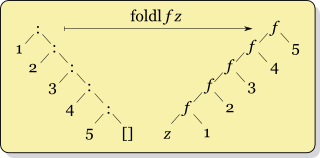
\includegraphics[width=0.5\textwidth]{fold_left}
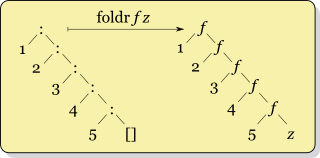
\includegraphics[width=0.5\textwidth]{fold_right}
\caption{Illustrations of fold left and fold right}
\label{fig:folds}
\end{figure}

We will now look into how we could implement this in Coq.

\subsection{Fold right} 
We implement fold right by matching on the input list. If the list is empty,
then we return the nil case. If the list is a head and a tail, we apply the cons
case to the head and call fold right recursive on the tail.

\subsection{Fold left}
We implement fold left by matching input list. If the list is empty, we
return the nil case. If the list is a head and a tail, we call fold left
recursive, where the nil case is replaced by an application of the cons case on
the head and the former nil case, and the list on which we now do the fold is
the tail of the list.

\section{A few functions}
In this chapter we will specify, define and implement a few different functions
using fold right and fold left. This will act as a stepping stone, while we are
learning to better understand fold right and fold left.

One should note that all of the following functions could be implemented without
using fold. But when we have the fold mechanism it turns out to be very easy to
implement these function as we will see.

\subsection{List identity}
We start with the simple example of the list identity function. The list
identity function takes a type and a list of that type, and returns the list it
is given.

We define the identity with fold right. The idea is that we let the cons case
function be the cons function, and the nil case be nil. In this way any input
list would simply be taken apart and be put back together by the fold.

We prove that it fits the specification with a simple structural induction
proof.

\subsection{List append}
In order to define a reverse list function, we will first need an implementation
of list append. We will also need append when we look It happens that we can
implement append with fold as well. The list append function takes a type and
two lists of that type, and returns a list where one has been appended on the
other.

We implement this almost like the list identity function, but this time we let
the nil case be the list that we want to append to the other. This means that
the first list is taken apart and constructed with the cons function, when we
reach nil, we replace it by the nil case which is the second list. In turn this
gives us exactly what we want.

Later on in our proofs about reverse, we will need the property that list append
is associative, in order to complete the proof. We prove this property using
structural induction on the first list.

\subsection{Reverse list}
With a specification and an implementation of list append, we are now in
position to define reverse list using fold. The reverse list function takes a
type and a list of that type and returns the reversed list.

This function is actually almost the same as the list identity function. The
only difference is that we use fold left instead of fold right. This means that
we take apart the list and then we construct it backwards. This in turn gives us
the reversed list.

The reason why we needed append is because the specification of reverse relies
on append. In fact we don't need an actual implementation of append at least not
in the proofs about reverse list. What we do need is the specification of
append. Because when we have the specification, we can just make an assumption
that we have an implementation, and the use this assumption to do the proof.

When we prove that this fold implementation of reverse fits the specification of
reverse, we need a master lemma in the cons case. The master lemma is the
following property about fold left: having a non-empty list as nil case is the
same as letting the nil case be nil and then append the list to the result of
the fold. This is proven by structural induction and with the help of the
property that append is associative.

We will see this pattern of using a master lemma in the cons case a few more
times in this project.

\subsection{Map}
In order to further explore how folds work, we decided to go a bit beyond the
project and look into map and a variation of it called map append. We start by
looking at the ordinary map function.

Map takes two types a function from the first to the second type and a list of
the first type.  It then returns a list where the function has been applied to
each element of the former list.

We implemented this using fold right. We let the cons case of the fold apply the
function to the current element, and we use cons to construct the new list.

\subsection{Map append}
Map append is a variation of map but where the function it is given always
returns a list. When we use an ordinary map, and the function that we give it
returns a list, then the result of the map will be a list of lists. Sometimes we
would rather have that we just got a flattened list back. This is exactly what
map append achieves.

The implementation looks a lot like the map implementation, but the key
difference is that we in the cons case have replace the list constructor with
our implementation of append. This means that in stead of constructing a list by
cons'ing lists together, we construct a list by appending lists together. In
turn this yields a flattened list instead of a list of lists.

\section{Back and forth}
In this chapter we will look at a connection between fold right and fold left.
We will in turn be able to define each in term of the other. We will do this
with an accumulator.

\subsection{Fold left from fold right}
We implement this by letting the fold have a nil case function which simply
returns what it is given. Lets call this function $n$

\begin{center}
  $n(a) = a$
\end{center}

And the cons case function which we will denote with a $c$, looks like this:

\begin{center}
  $c(x, h, a) = h (cons\_case(x, a))$
\end{center}

Please note that these are the functions we pass to fold right as nil case and
cons case, and the $cons\_case$ mentioned here is the one we would normally pass
to fold left. We know from the specification of folds that they return the same
type as their nil case, which means that when we give the above two to fold
right, the result will be a function taking one argument just like the nil case
function. This turns out to be a perfect fit for the function $h$.

In order to better explain this, consider the list $cons(1,cons(2, nil))$. 
\begin{align*}
        &fold\_left(nil\_case, cons\_case, cons(1,cons(2, nil))) 
  \\ &= fold\_right(n, c, cons(1,cons(2, nil)))(nil\_case)
  \\ &= (a \rightarrow c(1, fold\_right(n, c, cons(2,nil), a)))(nil\_case)
  \\ &= c(1, fold\_right(n, c, cons(2,nil), nil\_case))
  \\ &= fold\_right(n, c, cons(2,nil))(cons\_case(1,nil\_case))
  \\ &= fold\_right(n, c, nil)(cons\_case(2,cons\_case(1,nil\_case)))
  \\ &= n(cons\_case(2,cons\_case(1,nil\_case)))
  \\ &= cons\_case(2,cons\_case(1,nil\_case))
\end{align*}

In the final line we see that we get exactly what we would expect an ordinary
fold left would do.

Proving that this implementation of fold left fits the specification, and
thereby always \emph{acts} as a fold left is done by a simple structural 
induction proof on the input list.

\subsection{Fold right from fold left}
The implementation of fold right is very similar to that of the former fold left
implementation. $n$ and $c$ will remain the same, and if we do the same example
as the one above we get:
\begin{align*}
        &fold\_right(nil\_case, cons\_case, cons(1,cons(2, nil))) 
  \\ &= fold\_left(n, c, cons(1,cons(2, nil)))(nil\_case)
  \\ &= fold\_left((a \rightarrow c(1, n, a)), c, cons(2,nil))(nil\_case)
  \\ &= fold\_left((a \rightarrow n (cons\_case(1, a))), c, cons(2,nil))(nil\_case)
  \\ &= fold\_left((a \rightarrow cons\_case(1, a)), c, cons(2,nil))(nil\_case)
  \\ &= fold\_left((a \rightarrow (a \rightarrow 
  cons\_case(1,a))(cons\_case(2,a))), c, nil)(nil\_case)
  \\ &= (a \rightarrow (a \rightarrow
  cons\_case(1,a))(cons\_case(2,a)))(nil\_case)
  \\ &= (a \rightarrow cons\_case(1,a))(cons\_case(2, nil\_case))
  \\ &= cons\_case(1,cons\_case(2, nil\_case))
\end{align*}

Again we see that the result is what we would expect from a fold right.

In order to prover that this is the case for all lists and not just the one in
the example, we do a proof by structural induction on the list. Where the cons
case uses a master lemma.

\section{When cons case is an associative and commutative function}
When we wrote the code for the project, we noticed that some of the unit tests
for fold right and fold left were identical, and still passed for both of the
functions, while others only passed for one of them.

This happens when the cons case is an associative and commutative function.  In
order for the cons case function to be associative and commutative, it must take
two arguments of the same type. This means that if we can prove that the cons
case function is associative and commutative, then it should make no difference
whether we choose to use fold right or fold left --- The result should be the
same.

When we did the project we started by showing that the property held for plus as
the cons case function. We did this as stepping stone before writing a more
generalised version of the property. One should note that we choose to use ring
as the tactic that applies the associativity, commutativity and neutral element
rules. We could have written it out using the actual lemmas as well.  When
writing the generalised version, one sees that the actual proofs are more or
less the same thing.

\subsection{Structure of the proof}
The proof consists of a proof by structural induction on the input list.

In the cons case we will need a master lemma, which shows that after applying
the cons case for each of the folds once, fold right can then be replaced by
fold left.  The master lemma is also proven by structural induction. It is
reasonable to this nested induction because we will need three values in order
to apply the associativity rules.

The cons case of the master lemma is where we actually use the assumption that
the cons case function is associative and commutative, and that is really the
core of the proof.

\section{Primitive iteration and primitive recursion over polymorphic lists}
In the course for which this is a term project, we visited primitive recursion
and primitive iteration. In this chapter we will compare the two with fold left
and fold right.

The versions of primitive iteration and recursion that we looked at during the
course, worked on natural numbers. In order to compare with fold left and right,
we will need to specify and implement new versions of primitive iteration and
primitive recursion. First we will specify primitive iteration of polymorphic
lists, and compare this to fold left and fold right. Afterwards we will specify
primitive recursion over lists and do the same thing for that function.

\subsection{Primitive iteration over lists}
When we do primitive iteration over lists, we must define two things.
\begin{enumerate}
  \item What to do when the list is nil.
  \item What to do when the list consists of a head and a tail
\end{enumerate}

In the first case, we return what we what to happen when we reach nil. In the
second case, we return the result of applying a cons case function with the head
of the list as the first argument and in the second argument we call primitive
iteration recursively.

\subsubsection{Fold right from primitive iteration}
If we at this point stop and look at the specification of fold right, we will
see that the specifications are in fact the same thing. If we have an
implementation of primitive iteration, we can easily get an implementation of
fold right because primitive iteration also satisfies the specification of fold
right.

In fact this means that primitive iteration over lists is the same thing as fold
right.

\subsubsection{Fold left from primitive iteration}
We know that primitive iteration over list satisfies the specification of fold
right and earlier in the project we found a way of using a fold right to get a
fold left. If we combine this knowledge, we will have an implementation of fold
left from primitive iteration.

\subsection{Primitive recursion over lists}
Primitive recursion over lists is almost like the primitive iteration, only with
a slight change to the cons case function. The cons case function now takes one
more argument, which is a snapshot of the current list.

We can implement fold right and fold left in the exact same way as with
primitive iteration, if we just ignore that the snapshot exists.

\subsubsection{Usage of the snapshot}
This project was focused on folds, and we can easily implement folds without
using the snapshots. But in order to show some example usage of the snapshot in
primitive recursion, we implemented a function which maps a list to the list of
it's suffixes.

The last two unit tests for primitive recursion over lists show two functions
which make use of the snapshots. The first one returns a list of all the
snapshots, the second returns a flattened list of snapshots. We could specify,
and implement these functions if we were to expand on that topic.

We took a step further and defined three versions of the list of suffixes
function. Where one of these use the snapshot like the one in the unit test. The
other two are alternative implementations. We then prove these to be equivalent.

This is done by structual induction on the input list. When proving the
equivalency with the one that uses primitive iteration, we need a master lemma.
Apart from that the proof is straight forward.

\section{Conclusion}
In this report we looked at fold right and fold left. We saw that they share the
same expressive power, by showing that one could be defined in terms of the 
other. Afterwards we found out that when the cons case function that we pass
to a fold function is associative and commutative, then we get the same result
no matter if we use fold left or fold right. 

During this we saw a recurring proof pattern where we in the induction case of a
structural induction proof, needed a master lemma in order to complete the
proof.

In the end we saw that primitive iteration over lists is the exact same
thing as fold right. Using the connection between fold right and fold left, we
were able to define fold left in terms of primitive iteration. We also saw how
the snapshot in primitive recursion was irrelevant in relation to folding.

\end{document}
